\chapter{A Research Collaboration Recommender Based on Hybrid AI}\label{chap:ArtifactDevelopment}

This chapter presents the implementation of the proposed Knowledge-Driven and Hybrid \gls{ai} Architecture for Research Collaboration.
First of all, the technology stack used in the proposed system is described in Sec.~\ref{sec:technology-stack}.
Then, the process of populating the databases is explained in Sec.~\ref{sec:databases-population}.
Finally, the section \ref{sec:building-ai-agents} describes in detail the development of the agents and tools \gls{ai}, providing several examples of system use for each agent.

In the implementation phase, we addressed the third sub-research question:
\begin{center}
    \rqThree
\end{center}

\section{Technology Stack}\label{sec:technology-stack}
The proposed system is built entirely in \texttt{Python}, using \texttt{Streamlit} for both the back-end and front-end to simplify web app development and sharing.
\texttt{GraphDB}, developed by Ontotext, was chosen as the graph database for our system because of its robust support for the \gls{rdf} standard, enabling semantic data representation, efficient \gls{sparql} querying, and easy integration with \glspl{kg} for enhanced reasoning and retrieval.
Additionally, \texttt{Chroma} was selected as the vector database for storing \gls{kg} embeddings due to its efficient similarity search, scalable storage, and suitable integration with machine learning pipelines, ensuring fast and accurate retrieval of relevant entities.
To compute embeddings, we selected the \texttt{all-MiniLM-L6-v2} model due to its efficiency and strong performance in semantic similarity tasks.
This model is particularly well-suited for encoding short to medium-length text, making it ideal for our use case, where we store and retrieve project titles and abstracts from the \gls{eurio} dataset.
By leveraging a lightweight transformer architecture, \texttt{all-MiniLM-L6-v2} balances accuracy and computational efficiency, enabling fast and effective similarity search within our system.
To run the \texttt{all-MiniLM-L6-v2} model, we utilized \texttt{Ollama}, a lightweight, extensible framework for building and running language models on the local machine.
To implement our Graph\gls{rag} and Agentic\gls{rag} approach, we utilized two main frameworks: \texttt{LlamaIndex} was employed to build the agent workflow, coordinate agents, and integrate tools, while \texttt{LangChain} primarily facilitated the generation of \gls{sparql} queries from user query inputs.
For response generation, we utilized one of the state-of-the-art \glspl{llm}: \texttt{GPT-4o}, developed by OpenAI.
The context window and maximum output tokens for this model are detailed in Table~\ref{table:gpt-4o-tokens}, which illustrates its suitability for handling long input queries and generating high-quality responses.
The token limit represents the maximum number of tokens a model can handle in a single input, where a token typically corresponds to approximately \textsuperscript{3}/\textsubscript{4} of a word or four characters.

\begin{table}[htbp]
    \centering
    \scriptsize
    \begin{tabularx}{\textwidth}{|X|X|X|}
      \hline
      \textbf{Model} & \textbf{Context Window} & \textbf{Max Output Tokens}\\
      \hline
      GPT-4o 2024-05-13 & 128K tokens & 4,096 tokens\\
      \hline
    \end{tabularx}
    \caption{Context window and token limit of the GPT-4o model}
    \label{table:gpt-4o-tokens}
\end{table}

Finally, we containerized the entire system using \texttt{Docker} to ensure portability, reproducibility, and scalability across different environments.
Fig.~\ref{fig:proposed-system-graphRAG-technologies} provides a visual representation of the technologies used in the proposed system.

\begin{figure}[htbp]
    \centering
 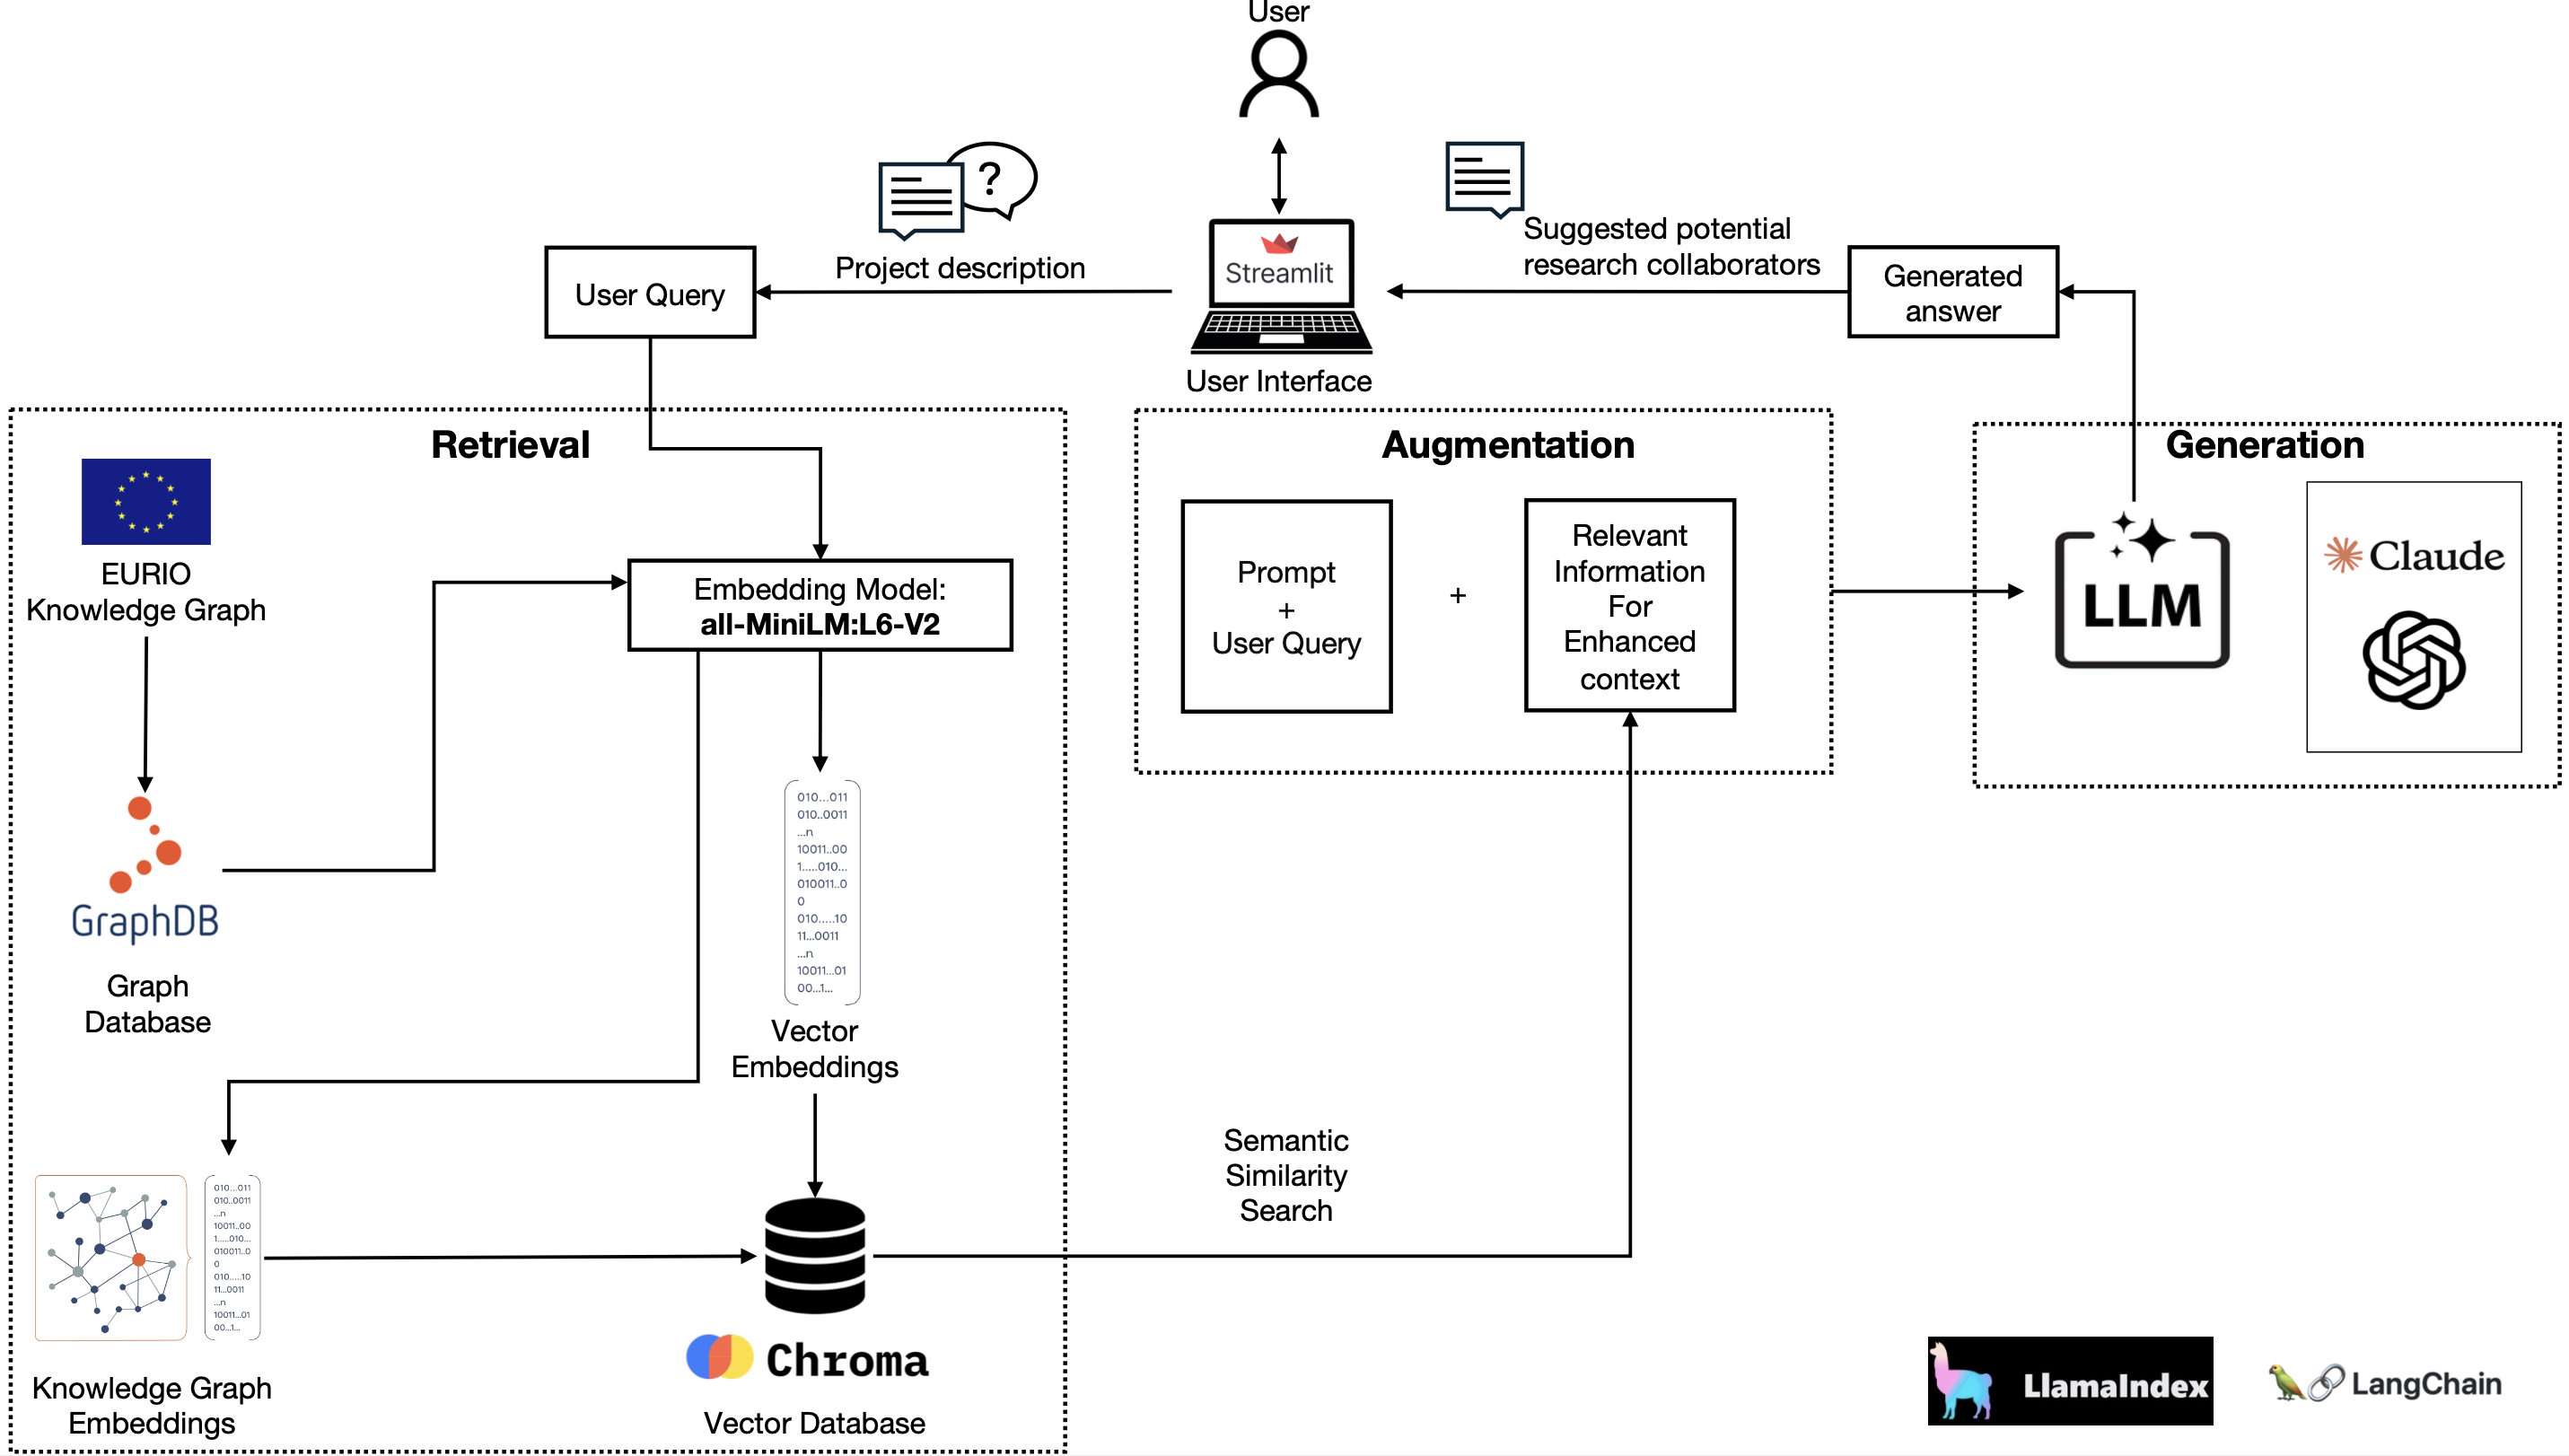
\includegraphics[width=.8\textwidth]{figures/implementation/proposed-system-graphRAG-technologies.png}
     \rule{35em}{0.5pt}
    \caption{Technologies used in the proposed Knowledge-Driven and Hybrid AI Architecture for Research Collaboration}
 \label{fig:proposed-system-graphRAG-technologies}
\end{figure}

The technology stack used in the proposed Knowledge-Driven and Hybrid \gls{ai} Architecture for Research Collaboration is summarized in Table~\ref{tab:technology-stack}.
The source code of the proposed recommender system is available on GitHub at \url{https://github.com/Piermuz7/MasterThesisProject.git}.

\begin{table}[htbp]
    \centering
    \scriptsize
    \begin{tabularx}{\textwidth}{|>{\centering\arraybackslash}p{2cm}|>{\centering\arraybackslash}p{2.5cm}|X|X|}
      \hline
      \textbf{Category} & \textbf{Technology/Tool} & \textbf{Description} & \textbf{Purpose/Usage} \\
        \hline
        Programming Languages & \texttt{Python} & A high-level, general-purpose programming language & Research Colaborator Recommender Development\\
        \hline
        Libraries & \texttt{Streamlit} & An open-source app framework for Machine Learning and Data Science projects & Front-end and back-end development\\
        \hline
        Graph Databases & \texttt{GraphDB} & A family of highly efficient, robust, and scalable \gls{rdf} databases & Knowledge Graph Population\\
        \hline
        Query Languages & \texttt{\gls{sparql}} & A query language and protocol for \gls{rdf} databases & Knowledge Graph Querying\\
        \hline
        Vector Databases & \texttt{Chroma} & An open-source vector database for storing and retrieve embeddings & Knowledge Graph Embeddings Storage\\
        \hline
        Embedding Models & \texttt{all-MiniLM-L6-v2} & A small but powerful model trained to generate high-quality sentence embeddings & Knowledge Graph Embeddings Generation\\
        \hline
        \glspl{llm} & \texttt{GPT-4o} & A multilingual, multimodal generative pre-trained transformer & Answer Generation in the \gls{rag} pipeline\\
        \hline
        Frameworks & \texttt{LangChain} & An open-source framework for developing applications powered by \glspl{llm} & \glspl{sparql} query generation in \gls{rag} pipeline development\\
        \hline
        Frameworks & \texttt{LlamaIndex} & An open source data orchestration framework for building applications based on \glspl{llm} & Agent Workflow in \gls{rag} pipeline development\\
        \hline
        Frameworks & \texttt{Ollama} & A lightweight, extensible framework for building and running language models on the local machine & Used to run all-MiniLM-L6-v2\\
        \hline
        Containerization and Deployment & \texttt{Docker} & An open platform for developing, shipping, and running applications & Containerization of the entire system\\
        \hline
    \end{tabularx}
    \caption{Technology stack used in the proposed Knowledge-Driven and Hybrid \gls{ai} Architecture for Research Collaboration}
    \label{tab:technology-stack}
\end{table}

\section{Databases Population}\label{sec:databases-population}
The first step is populating the databases, which involves importing the \gls{eurio} \gls{kg}, provided in \gls{rdf} N-Quad format, into GraphDB.
This process ensures that the structured knowledge about EU-funded research projects is stored in a graph database, allowing for efficient querying and retrieval of relevant information.
During the \acrlong{kg} Exploration (Sec.~\ref{sec:ontology-selection}), it was observed that not all projects within the \gls{eurio} dataset have associated participants.
In other words, several projects exist in the \gls{kg} without any recorded participants.
Given that the goal of the system is to recommend research collaborators based on project involvement, it is crucial to ensure that only relevant data is processed in the embedding generation phase.
To maintain efficiency and relevance, embeddings of title and abstract are computed only for projects that have at least one associated participant.
This is achieved by filtering out projects without participants using the \gls{sparql} query shown in Listing~\ref{lst:projects-with-at-least-one-participants}.

\begin{lstlisting}[language=SPARQL, caption={\gls{sparql} query for getting the projects with at least one participant}, label={lst:projects-with-at-least-one-participants}]
    PREFIX eurio: <http://data.europa.eu/s66#>
    PREFIX rdfs: <http://www.w3.org/2000/01/rdf-schema#>
    SELECT DISTINCT ?project ?title ?abstract
    WHERE {
        ?project a eurio:Project .
        ?project eurio:title ?title .
        ?project eurio:abstract ?abstract .
        FILTER EXISTS {
            ?project eurio:hasInvolvedParty ?party .
            ?party a eurio:OrganisationRole .
            ?party eurio:isRoleOf ?role .
            ?person eurio:isInvolvedIn ?project .
            ?person eurio:isEmployedBy ?role .
            ?person eurio:isRoleOf ?p .
        }
    }
\end{lstlisting}

The query \gls{sparql} returned 25,482 projects with at least one participant involved in each project.
Of these projects, title and abstract embeddings were calculated and stored in the Chroma vector database.
In this way, the vector database contains only meaningful representations of research projects with involved participants, avoiding unnecessary computations for projects without involved participant.
Since the \gls{kg} is too large to process in a single step, embeddings were stored in Chroma in batches of 1,000 entities at a time to efficiently manage memory usage and avoid performance bottlenecks.

\section{Building AI Agents and Tools}\label{sec:building-ai-agents}
Once the \gls{kg} and related embeddings are stored in the databases, we need to implement the system's core functionalities.
This involves building \gls{ai} agents and tools to facilitate the recommendation process.
As described in Sec.~\ref{sec:architecture-design}, the user interface is designed as a chatbot, where users can interact with the system by asking questions and receiving responses.
To enable this interaction, we developed three main agents and five different tools.
The agents are responsible for coordinating the workflow, generating responses, and managing the system's overall functionality.
The tools, on the other hand, are designed to perform specific tasks, such as generating \gls{sparql} queries, extracting relevant information, and providing recommendations.
\textbf{LlamaIndex} is used to set a prompt to agents, which instructs agents to execute specific tools, respond according to a certain format, and so on.
\textbf{Langchain}, on the other hand, is used exclusively for generating \gls{sparql} queries based on user input.
The data returned from these queries will then be used in turn by the agents.
The agents and tools are described in more detail below.
For readability, only the agents' prompt templates are provided in the appendices, and the tool names used in this thesis differ from those in the prompt templates.

\subsection*{Project-Participants-Information Agent}
The process starts with a user query, which is handled by a coordinator agent, also called master agent.
This agent act as central orchestrator, executing specific tasks, or assigning the query to specialized retrieval agents according to its specific requirements.
In other words, this agent is tasked with retrieving information on projects and participants.
It is equipped with a prompt template that it must follow.
The prompt, shown in Appendix~\ref{app:ProjectParticipantsAgent}, sets the scope of the master agent, making it explicit that it must answer purely related questions in the context of European projects.
With this prompt, the agent is instructed on how to use its tools: \textit{Project information} and \textit{Project participants}.
The first tool has its own prompt template, which contains example \gls{sparql} queries to generate a \gls{sparql} query from the user input.
Once the query is generated, the agent will use it to query the \gls{kg} and retrieve the relevant information.
The agent will then use the information to generate a response to the user query.
For example, if the user asks for the relative information of a project entitled ``Knowledge-Based Information Agent with Social Competence and Human Interaction Capabilities'', the agent will use this tool to generate the \gls{sparql} query shown in Listing~\ref{lst:project-information-sparql-query}.

\begin{lstlisting}[language=SPARQL, caption={\gls{sparql} query for getting information of a project entitled ``Knowledge-Based Information Agent with Social Competence and Human Interaction''}, label={lst:project-information-sparql-query}]
PREFIX eurio: <http://data.europa.eu/s66#>
SELECT DISTINCT ?title ?url ?abstract ?status ?startDate ?endDate
WHERE{
    ?project a eurio:Project .
    ?project eurio:title "Knowledge-Based Information Agent with Social Competence and Human Interaction Capabilities" .
    ?project eurio:title ?title .
    ?project eurio:url ?url .
    ?project eurio:abstract ?abstract .
    ?project eurio:projectStatus ?status .
    ?project eurio:startDate ?startDate .
    ?project eurio:endDate ?endDate .
}
\end{lstlisting}

Once, the information is retrieved, the agent will use its prompt template to generate a response with such information.

The second tool also has its own template with SPARQL queries to follow as an example for generating queries to obtain information on participants.
An example query set in the prompt of this tool is shown as follows.
If the user asks ``Who is Emanuela Merelli?'', the agent will use this tool to generate the \gls{sparql} query shown in Listing~\ref{lst:person-information-sparql-query}.
This query retrieves information about a person named Emanuela Merelli, including their organization, contact details, and projects they are involved in.

\begin{lstlisting}[language=SPARQL, caption={\gls{sparql} query for getting information of a person}, label={lst:person-information-sparql-query}]
PREFIX eurio: <http://data.europa.eu/s66#>
PREFIX rdfs: <http://www.w3.org/2000/01/rdf-schema#>
SELECT ?person_label ?org_name ?telephone ?fax ?project_title
WHERE {
    ?person a eurio:Person .
    ?person rdfs:label ?person_label .
    ?person eurio:hasContactDetails ?contact_details .
    ?contact_details eurio:telephone ?telephone .
    OPTIONAL{{?contact_details eurio:faxNumber ?fax .}}
    FILTER (LCASE(?person_label) = "emanuela merelli") .
    ?person eurio:hasRole ?role .
    ?role eurio:isEmployedBy ?org .
    ?org rdfs:label ?org_name .
    ?role eurio:isInvolvedIn ?project .
    ?project a eurio:Project .
    ?project eurio:title ?project_title .
}
\end{lstlisting}

Fig.~\ref{fig:example-who-is-emanuela-merelli} shows an example of a user query asking for information about a person named Emanuela Merelli, using the chatbot interface.

\begin{figure}[htbp]
    \centering
 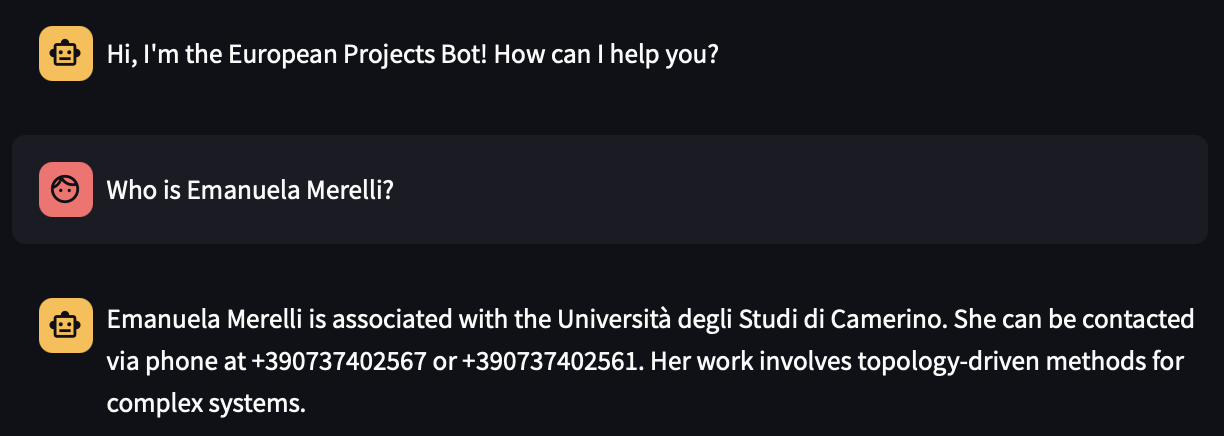
\includegraphics[width=.75\textwidth]{figures/implementation/example-who-is-emanuela-merelli.png}
     \rule{35em}{0.5pt}
    \caption{Example of a user query asking for information about a person named Emanuela Merelli}
 \label{fig:example-who-is-emanuela-merelli}
\end{figure}

Fig.~\ref{fig:example-general-info-about-topology-driven-methods-for-complex-systems-project} shows another example of a user query asking for information about a project entitled ``Topology-Driven Methods for Complex Systems''.
This query is handled by the same agent, which uses the \textit{Project information} tool to generate the \gls{sparql} query to retrieve the project's metadata.
The chatbot's response presents the abstract of the project and briefly explains which topics it focused on and the types of scientists involved.
However, it does not mention the researchers involved, because the \textit{Project participnats} tool was not used.
Finally, the duration and two useful links related to the project are given.

\begin{figure}[htbp]
    \centering
 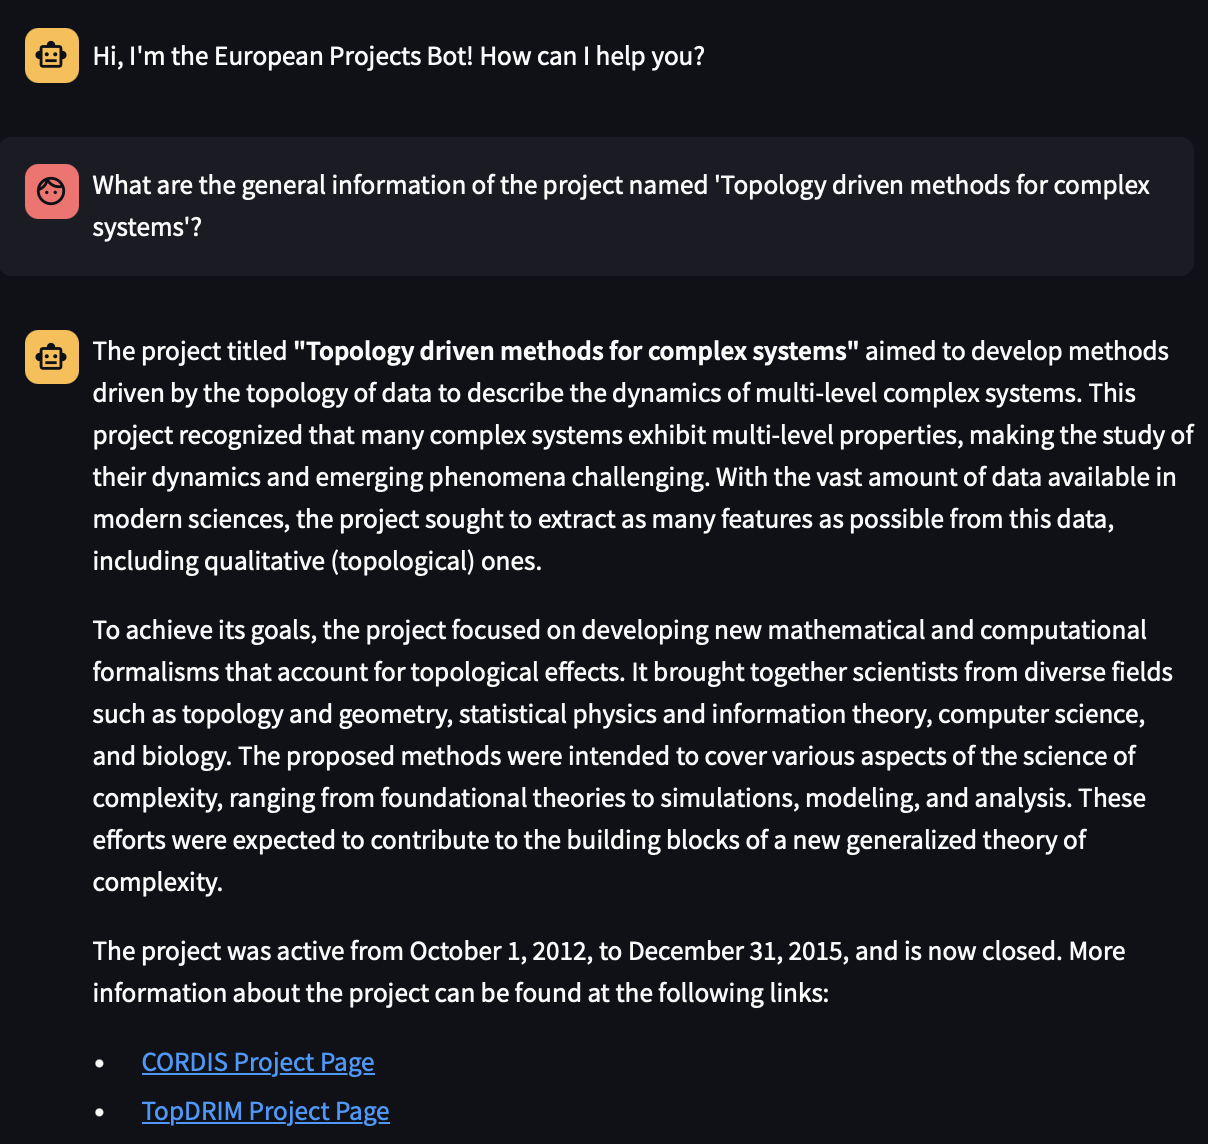
\includegraphics[width=.8\textwidth]{figures/implementation/example-general-info-about-topology-driven-methods-for-complex-systems-project.png}
     \rule{35em}{0.5pt}
    \caption{Example of a user query asking for information about a project entitled ``Topology-Driven Methods for Complex Systems''}
 \label{fig:example-general-info-about-topology-driven-methods-for-complex-systems-project}
\end{figure}

Fig.~\ref{fig:example-participants-of-topology-driven-methods-for-complex-systems-project} shows an example of a user query asking for information about participants involved in the same project of Fig.~\ref{fig:example-general-info-about-topology-driven-methods-for-complex-systems-project}.
This user input query is handled by the same agent, which will use the \textit{Project participants} tool to generate the \gls{sparql} query in order to retrieve the project's participants.
In this example, the project coordinator and the 5 participants involved are listed.
Moreover, the organization where this participant is employed, along with its full postal address, is provided to ensure accurate identification and location details.

\begin{figure}[htbp]
    \centering
 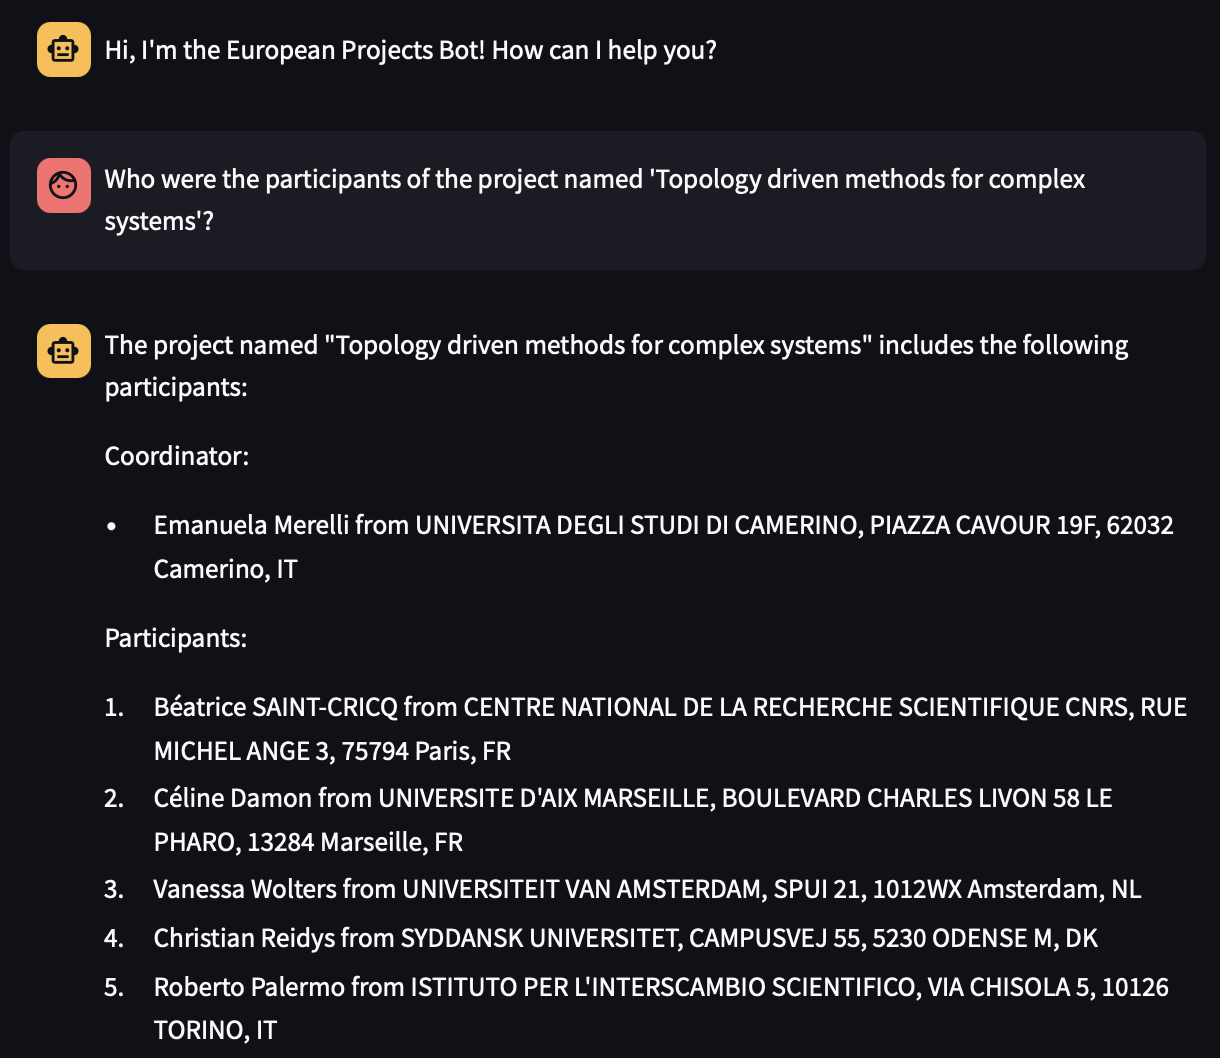
\includegraphics[width=.75\textwidth]{figures/implementation/example-participants-of-topology-driven-methods-for-complex-systems-project.png}
     \rule{35em}{0.5pt}
    \caption{Example of a user query asking for information about participants in a project entitled ``Topology-Driven Methods for Complex Systems''}
 \label{fig:example-participants-of-topology-driven-methods-for-complex-systems-project}
\end{figure}

In addition to retrieve project and participant information, the master agent can delegate user queries to other specialised agents.
If it is inferred from the user input that the task to be performed is to suggest collaborators for a project description and objectives given as input, then the master agent will delegate this task to the \textit{Potential Collaborators Agent}.
Otherwise, if the task is to suggest potential consortium organisations for a project description and objectives given as input, then the master agent will delegate this task to the \textit{Potential Consortium Organisations Agent}.

\subsection*{Potential Collaborators Agent}
This agent recommends potential research collaborators based on a given project description and objectives.
It is instructed via the prompt template shown in Appendix~\ref{app:PotentialCollaboratorsAgent}, in order to follow a structured process to identify relevant collaborators by leveraging existing project data, retrieving information about researchers, and refining its recommendations using web-based sources.
Unlike the master agent, this agent does not use prompts to generate \gls{sparql} queries from user input.
The process begins with analyzing the given project description to extract its main concepts.
This is a starting point to identify relevant past projects and researchers.
To find similar projects, the agent searches for previously funded projects with abstracts similar to the given description.
The retrieved information includes project metadata such as the project title, abstract, URI, and other relevant details.
Once similar projects have been identified, the agent proceeds to find collaborators associated with these projects.
This step involves extracting information about researchers who have contributed to the identified projects.
The agent ensures that all project URIs obtained from the similarity search are used to gather a comprehensive list of potential collaborators.
For each collaborator, key details such as their full name, affiliated organization, and past project involvement are retrieved.
As mentioned earlier, the names of the tools in the thesis are not the same at code level.
The process of how contributors are extracted to suggest described so far, is equivalent to the \textit{Recommend collaborators} tool.
After generating an initial list of potential collaborators, the agent uses the \textit{Search Web} tool to gather additional information about their research areas and expertise.
To enhance the quality and relevance of the recommendations, the agent formulates a set of keywords summarizing each collaborator's research topics.
This web search is performed only if potential collaborators have been found.
The final output consists of a structured list of recommended collaborators, each including the researcher's full name, affiliated organization with postal address, the title of a relevant past project, and keywords summarizing their research areas.
This format provides clarity and usability for users looking for opportunities for research collaboration.
If no similar projects or collaborators are found, the agent does not proceed with web searches.
Instead, it provides a professional response explaining that no relevant matches were identified.

\begin{figure}[h]
    \centering
    \begin{subfigure}{0.45\textwidth}
        \centering
        
\includegraphics[width=.7\textwidth]{figures/implementation/example-collaborators-recommendation-question.png}
        \caption{}
        \label{fig:example-collaborators-question}
    \end{subfigure}
    \hfill
    \begin{subfigure}{0.45\textwidth}
        \centering
        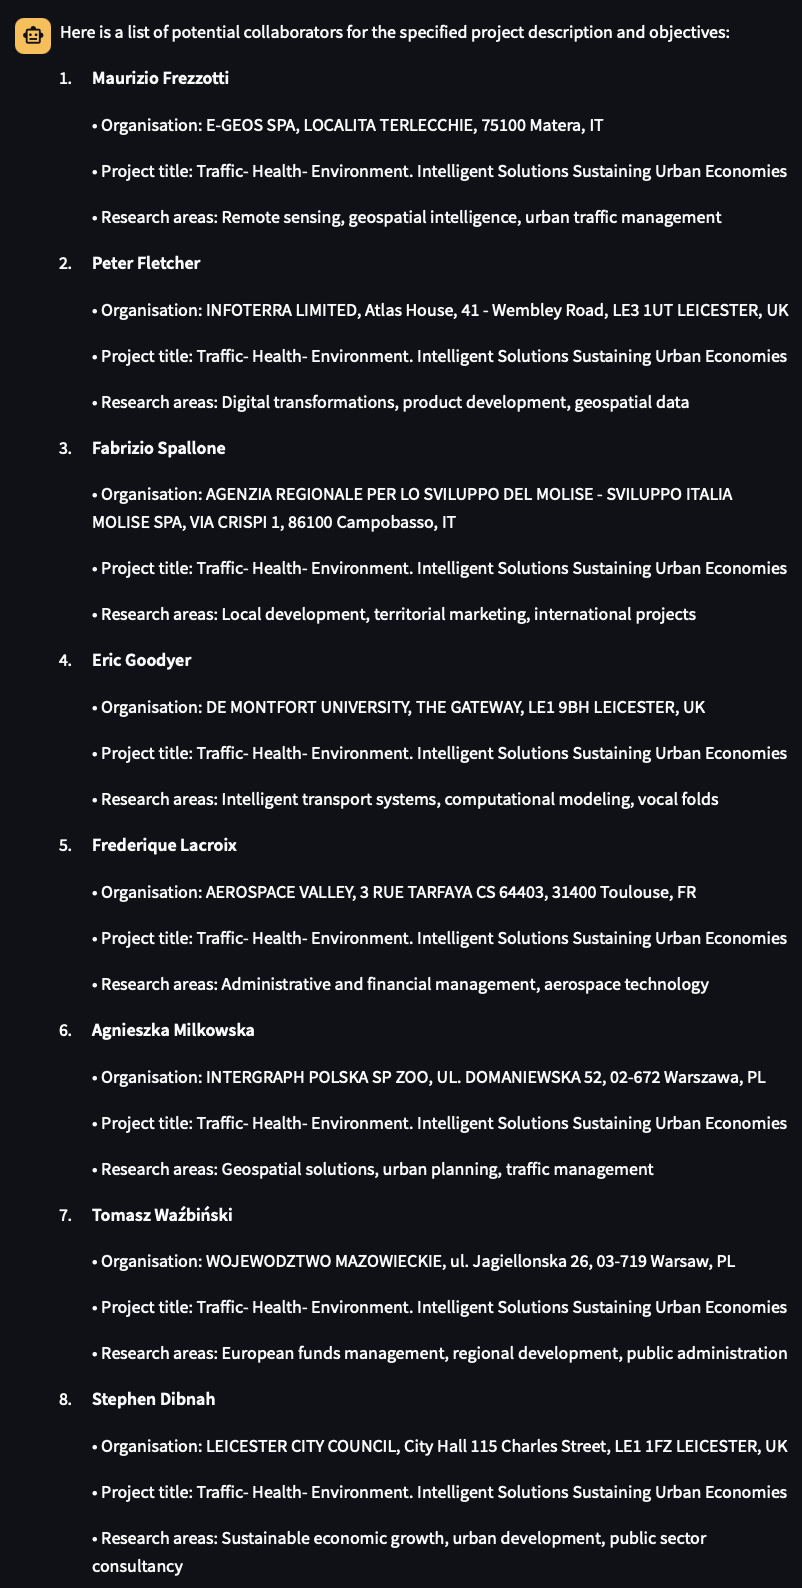
\includegraphics[width=.6\textwidth]{figures/implementation/example-collaborators-recommendation-answer.png}
        \caption{}
        \label{fig:example-collaborators-answer}
    \end{subfigure}
    \rule{35em}{0.5pt}
    \caption{(\subref{fig:example-collaborators-question}): The user need is to find potential collaborators for a project description and objectives.
    (\subref{fig:example-collaborators-answer}): The chatbot response with the list of potential collaborators.}
    \label{fig:example-collaborators-recommendation}
\end{figure}

An example of a user query asking for potential collaborators for a project description and objectives is shown in Fig.~\ref{fig:example-collaborators-recommendation}.
The user query is handled by the \textit{Potential Collaborators Agent}, which uses the \textit{Recommend collaborators} tool to retrieve the potential collaborators.
The chatbot's response presents a list of potential collaborators, including their full names, affiliated organizations, and past project involvements.
Since the response is too long to fit in a single screenshot, only the first few collaborators are shown in the response.

\subsection*{Potential Consortium Organisations Agent}
Finally, this agent recommends potential consortia based on a given project description and objectives.
It is instructed through the detailed prompt in Appendix~\ref{app:PotentialConsortiumOrganisationsAgent} to suggest potential organisations that could form a consortium for a given project.
The agent follows a multi-step approach to identify relevant organisations based on similar projects and their associated participants.
Its prompt provides a clear sequence of tasks that the agent must follow.
First, it processes the user-provided project description and objectives to extract key concepts and requirements.
It then queries the database to identify projects with abstracts similar to the given project description.
These similar projects provide context for selecting relevant organisations.
Once similar projects are found, it extracts the organisations involved in those projects.
After retrieving this information, the agent organizes the organisations into one or more consortium lists, ensuring that each consortium includes at least four organisations with distinct contributions, that no organisations are repeated within the same consortium, and that each organisation has a clearly defined role based on its past research.
For each organisation, the agent specifies its postal address, explains its potential contribution to the project by linking it to specific project objectives, and lists its related works extracted from previous projects to justify its relevance.
For the same reason as the consistency of tool names, the explanation given so far of the suggestion of consortia is equivalent to the \textit{Recommend consortium organisations} tool.
Once the consortia list is constructed, the agent may use the \textit{Search Web} tool to get additional details on the organisations' research areas.
However, this step is only executed if similar projects and organisations are found.
The prompt is a highly structured instruction set designed to guide the agent in generating well-justified and relevant consortium recommendations.
It outlines the input format, the retrieval process, and the expected output structure.
The agent is given a clear goal: to suggest organisations suitable for forming a consortium based on a project description.
An example input format is provided to clarify how the agent should interpret user queries.
The output format is strictly defined, requiring the agent to provide each organisation's name, postal address, potential contribution with references to project objectives, and a list of related works detailing past projects where the organisation was involved.
As a matter of quality and consistency, the agent must avoid selecting overly similar organisations while assembling teams that provide complementary skills and expertise.
If no relevant organisations are found, it must generate a professional response explaining the absence of suitable matches without invoking external knowledge.

Fig.~\ref{fig:example-consortium-organisations-recommendation-question} shows an example of a user query asking for potential consortium organisations for a project description and objectives, as those in Fig.~\ref{fig:example-collaborators-question}.

\begin{figure}[htbp]
    \centering
 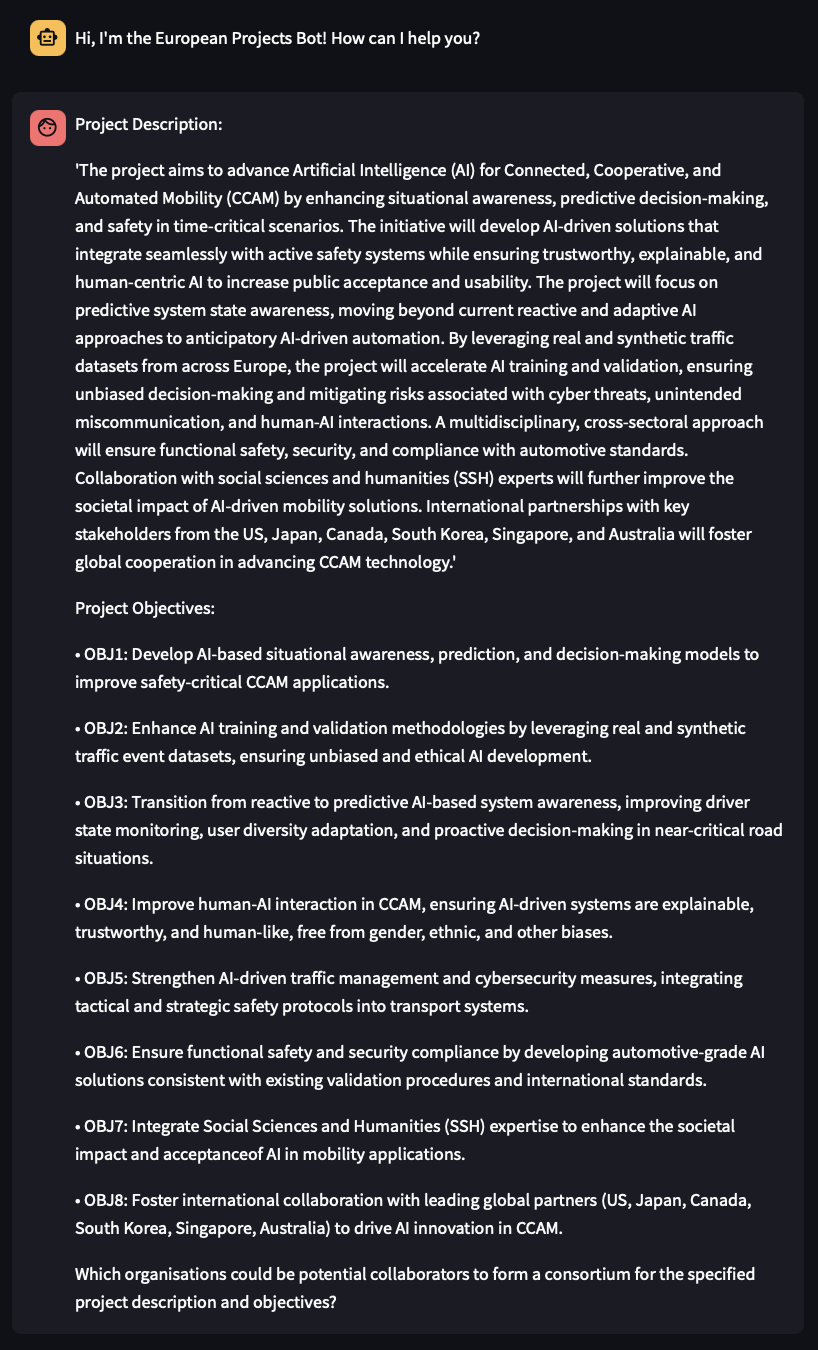
\includegraphics[width=.4\textwidth]{figures/implementation/example-consortium-organisations-recommendation-question.png}
     \rule{35em}{0.5pt}
    \caption{Example of a user query asking for potential consortium organisations for a project description and objectives}
 \label{fig:example-consortium-organisations-recommendation-question}
\end{figure}

The user query is handled by the \textit{Potential Consortium Organisations Agent}, which uses the \textit{Recommend consortium organisations} tool to retrieve the potential consortium organisations.
As shown in Fig.~\ref{fig:example-consortium-organisations-recommendation-answer}, the chatbot's response presents a list of potential consortium organisations is presented in the chatbot's response, including their names, postal addresses, potential contributions, and related works.
There are two consortium lists, each containing five organisations with distinct contributions.

\begin{figure}[h]
    \centering
    \begin{subfigure}{0.45\textwidth}
        \centering
        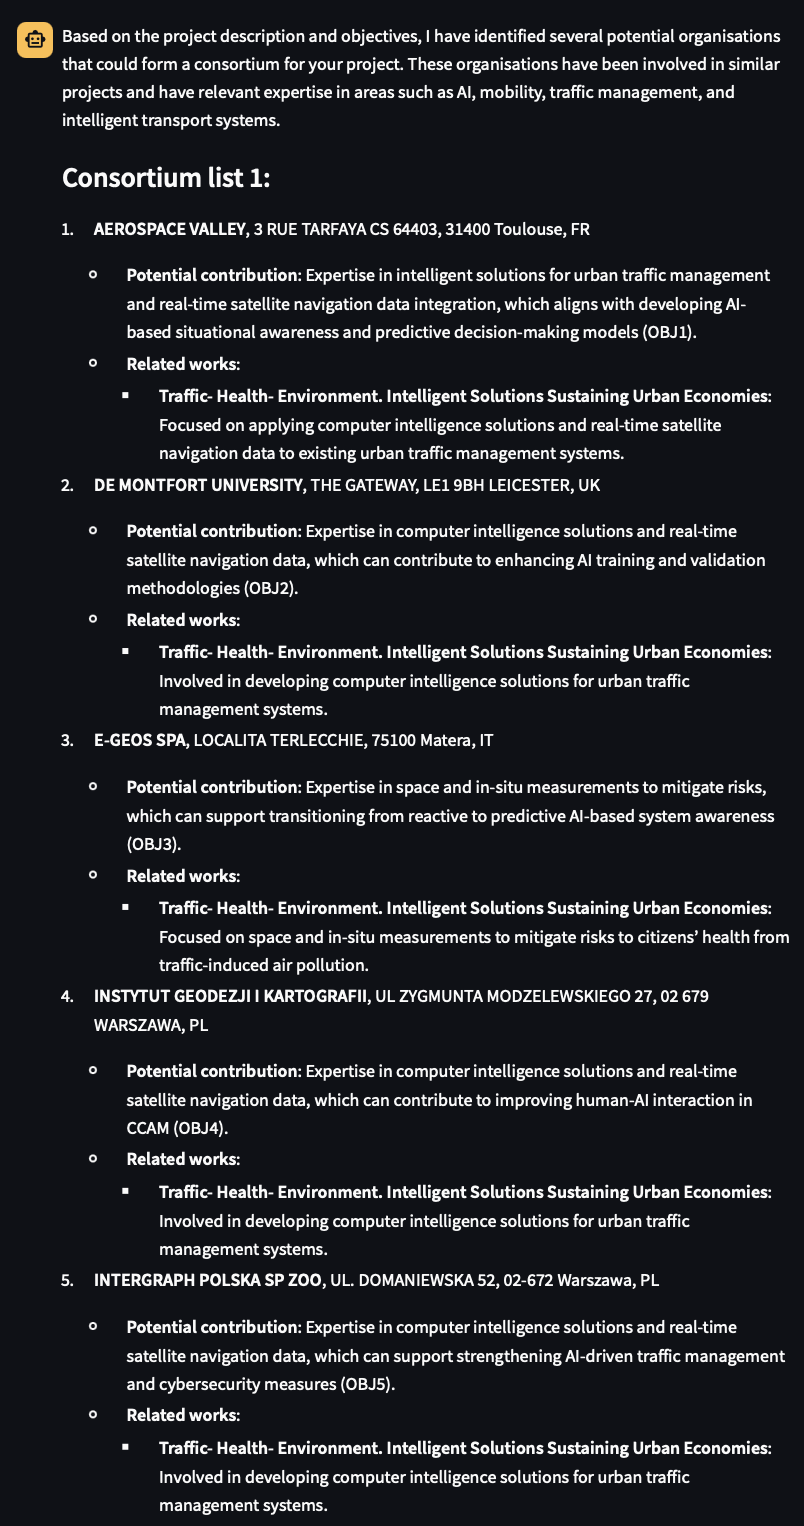
\includegraphics[width=.8\textwidth]{figures/implementation/example-consortium-organisations-recommendation-answer-pt1.png}
        \caption{}
        \label{fig:example-consortium-organisations-recommendation-answer-pt1}
    \end{subfigure}
    \hfill
    \begin{subfigure}{0.45\textwidth}
        \centering
        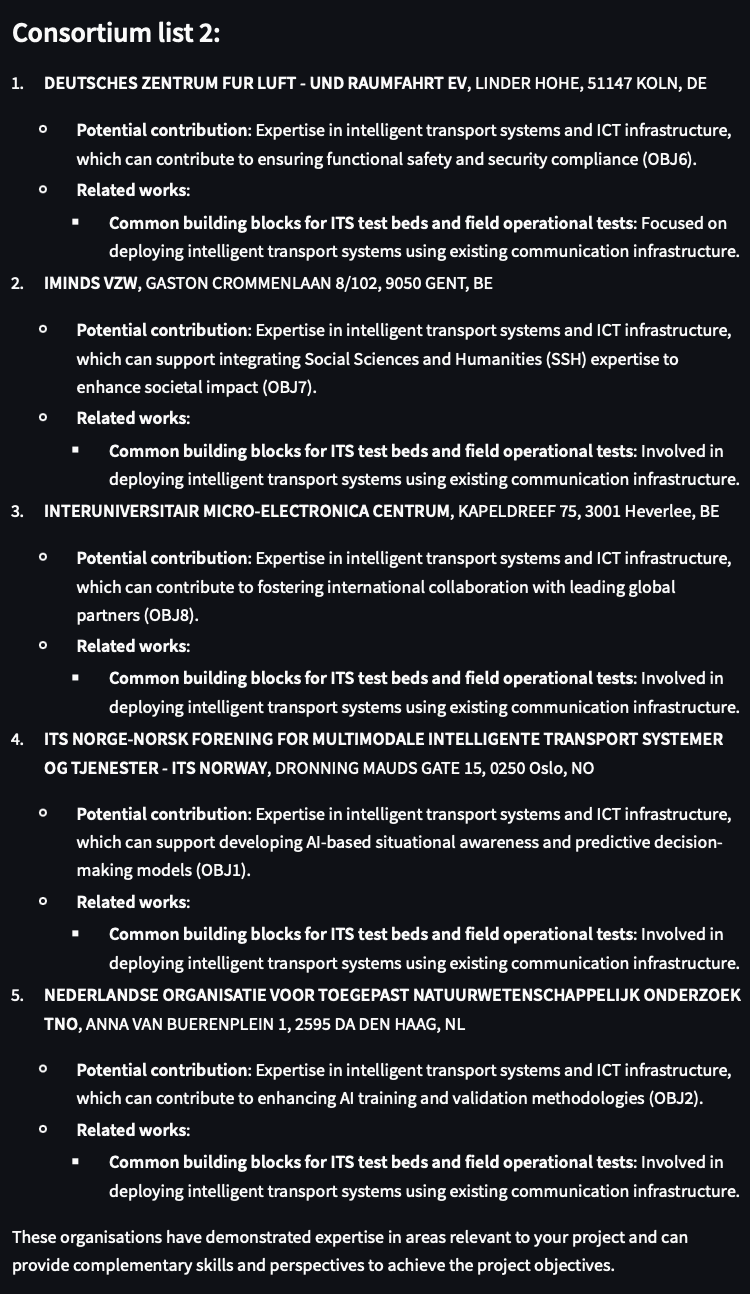
\includegraphics[width=.8\textwidth]{figures/implementation/example-consortium-organisations-recommendation-answer-pt2.png}
        \caption{}
        \label{fig:example-consortium-organisations-recommendation-answer-pt2}
    \end{subfigure}
    \rule{35em}{0.5pt}
    \caption{(\subref{fig:example-consortium-organisations-recommendation-answer-pt1}): The chatbot response with the list of potential organisations of Consortium list 1.
    (\subref{fig:example-consortium-organisations-recommendation-answer-pt2}): The chatbot response with the list of potential organisations of Consortium list 2.}
    \label{fig:example-consortium-organisations-recommendation-answer}
\end{figure}